%!TEX root = ../Thesis.tex

\section{Planar Assumption Analysis}
\subsection{Setup}
These results had no error induced in the measurements in order to analyse the effectiveness and robustness of the algorithm. No epoch alignment and no correlated or uncorrelated errors. Only two receivers were used with the reference receiver exactly at the approximate location. The second receiver was set at varied configurations of a set distance north, east and down of the reference receiver. The set distance between the receivers was varied from 1 mm to 100 km. As there are no randomly induced errors, there is no statistical analysis. The algorithm was also adjusted to not solve for a clock bias variable to see how the least squares solution adjusted the distance between planes without error in the system.\\

The satellites were configured in a small cluster to analyse how the position of the satellites relative to the configuration of the receivers affected the plane assumption. The total error and the individual component error were calculated to identify what component produces the most error for the configuration.\\

This analysis was not required to be compared to NLLS as there was no error and it would solve the system perfectly to mathematical precision.

\subsection{Discussion}
See Figure \ref{fig:plane_ALLE_north_9060}, two receiver configuration with one receiver at the approximate location and one receiver at varying distance along the north direction. The cluster of satellites were set perpendicular to the receiver configuration as it was predicted to be a configuration with less error. This isolated the error due to the plane assumption. The algorithm was compared to solving the same plane intersections but without the clock bias variable. In Figure \ref{fig:plane_ALLE_north_9060}, for distances < 1 meter, the planar algorithm solution has a consistent error two orders of magnitude larger than the solution without the clock bias. This indicates that without errors, the least squares matrix adjusts the distance between planes proportionally but will introduce errors. These errors however are on the order of micrometers ($10^{-6}$) and will be below the noise floor with any error in the system.\\

The results show that the least squares setup by constraining to the reference receiver is successful as the error is not proportional to distance below 10 m. Above 10 m the error increases for both the solutions with and without the clock bias, indicating that the error is due to the planar assumption. The slope has a gradient of $m = \log(10^4)/\log(10^2) = 2$ which means the error is proportional to the square of the distance. This was to be expected as in reality, the distance from the satellites are spheres, as stated in Eq\eqref{Eq:squarerel}. However the magnitude of error was 1 m at 10 km distance, which for localised systems is acceptable.\\

The individual component error shows where the error has come from. In Figure \ref{fig:plane_ALLE_north_9060}, it the error in the north component is much smaller than the error due to the east or down component. This is based on the satellite configuration relative to the receiver configuration, however in this case it can be misleading. As the satellite cluster is directly east of the reference receiver at a high elevation, the error due to the plane assumption bends towards the east and up. This is also evident in Figure \ref{fig:plane_ALLE_north_0075} where the satellite configuration is directly north of the system. The east direction has the least amount of error for the same reason. A full analysis of the effect of the satellite configuration was conducted for each two receiver configuration.\\


%% using main_fn.m
\begin{figure}
\centering
\caption[Error of Plane Assumption vs Distance along North vector]{Error of Plane Assumption vs Distance along North vector. \textbf{Top Left}: Receiver configuration in NED of the approximate location. One receiver at the center and one along the north vector. \textbf{Bottom Left}: Satellite configuration. Cluster of 5 satellites around elevation $60^\circ$ and azimuth $90^\circ$. \textbf{Top Right}: Magnitude of total error vs the distance between receivers with and without solving for the clock bias. \textbf{Bottom Right}: North/East/Down error components vs the distance between receivers.}
\label{fig:plane_ALLE_north_9060}
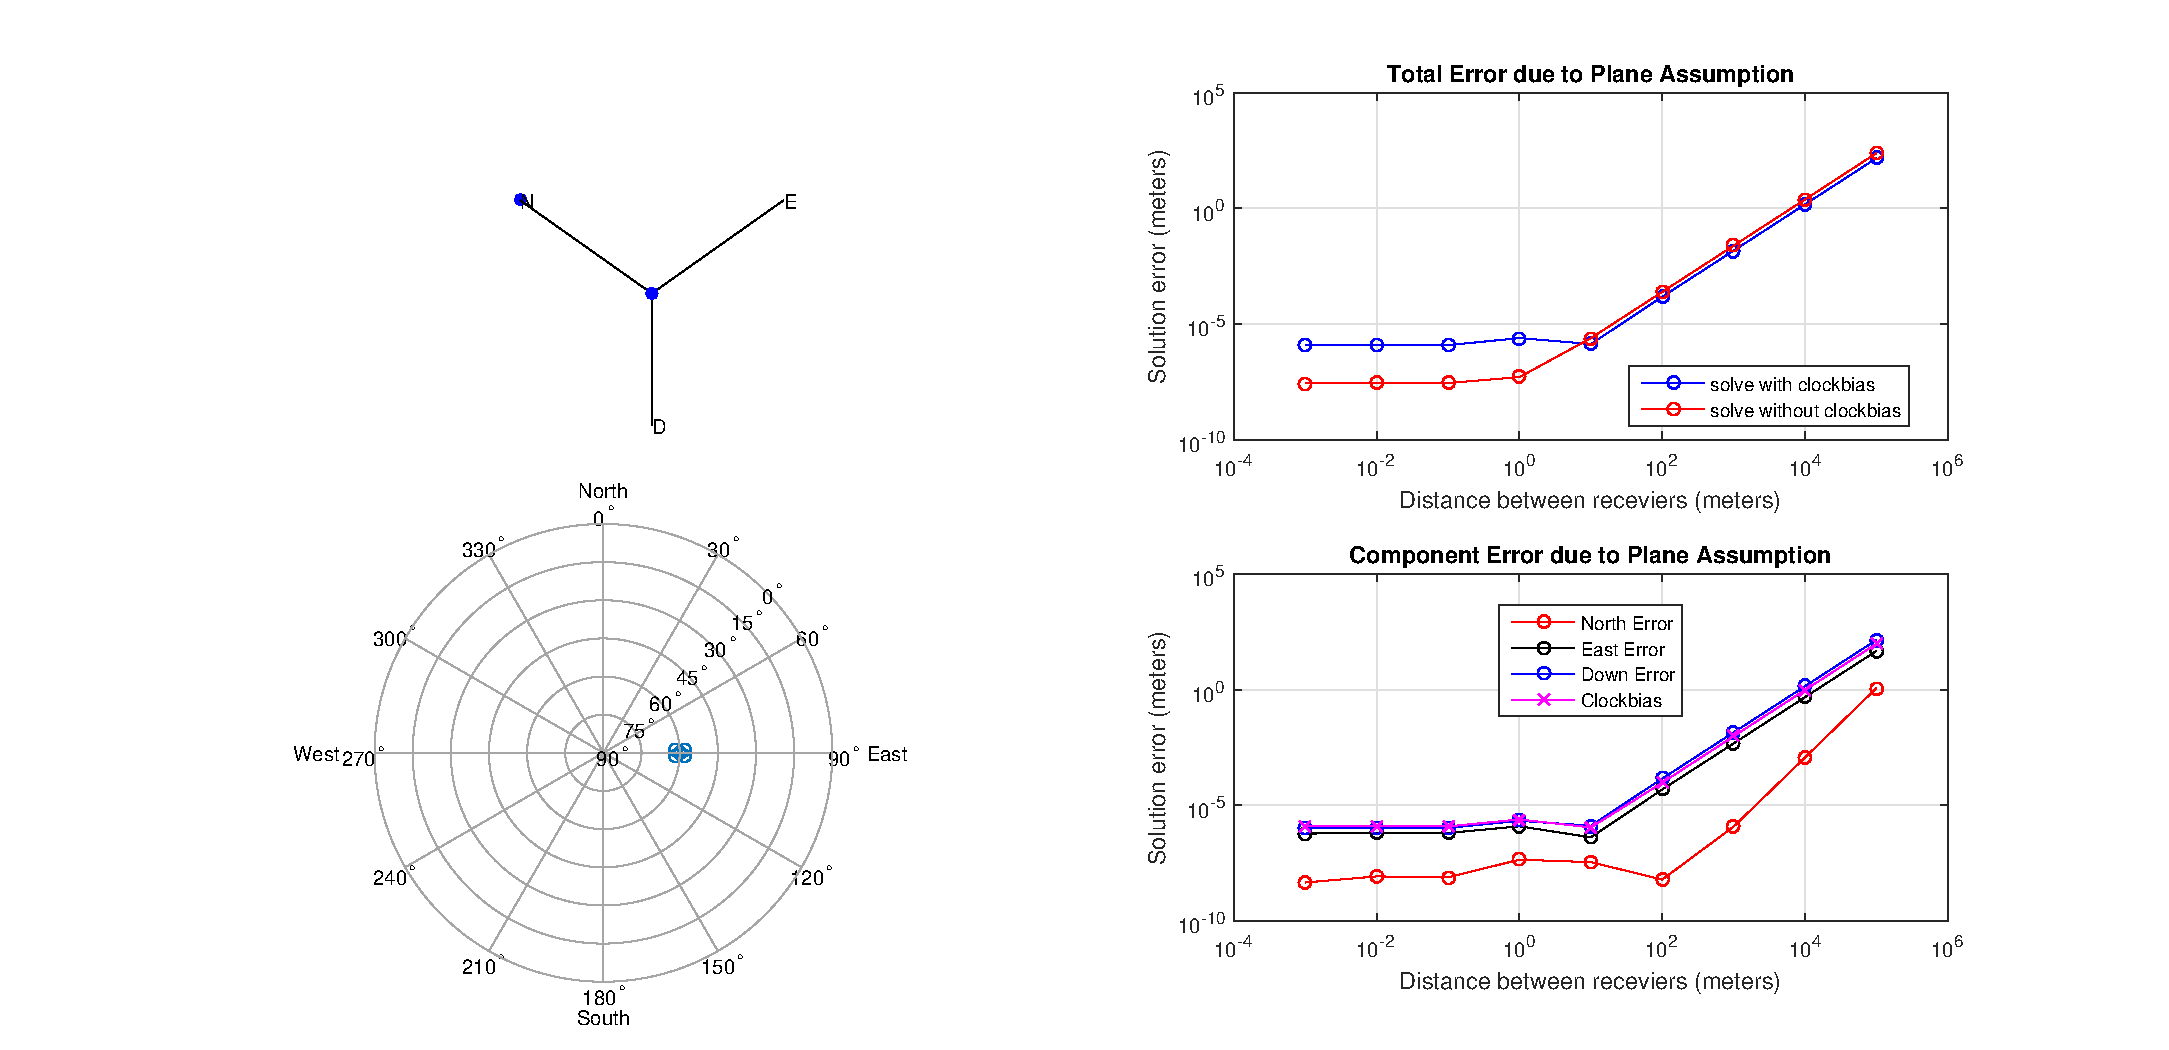
\includegraphics[trim = 3cm 0 0 0,clip,width=\linewidth]{ChapterExperiments/Figures/plane_ALLE_north_9060}
\end{figure}

The total error based on satellite configuration shown in Figure \ref{fig:plane_total_north1_pow4} for Northerly displaced receivers, Figure \ref{fig:plane_total_east_pow4} for East and Figure \ref{fig:plane_total_down_pow4} for Down. Note that the minimum for the Down configuration was 2 m whereas the minimum for the horizontal was 0.5 m. The down vector will inherently will have more error as the sphere curves up away from the plane assumption, however it is still in the same magnitude. It is due to the nature of the system, that the satellites are above the Earth, that PNT has less accuracy in the vertical plane than the horizontal plane as stated by the SPS Performance Standard \cite{officalperformance}. The north and east configurations are the same but $90^\circ$ out of phase. A full breakdown of which component causes the error is shown in Figure \ref{fig:plane_fullbreakdown}. High elevation causes the most error for both configurations, due to the down component, see (e) and (f) of Figure \ref{fig:plane_fullbreakdown}. The large error along the axis of the horizontal displacement, that is north for north and east for east, was due to the same direction, see (a). The orthogonal direction contributed significantly less error.\\

Based on this information, a satellite configuration was created to minimise the error due to the plane assumption in order to explore other affects.


\begin{figure}
\centering
\caption{}
\label{fig:plane_ALLE_north_0075}
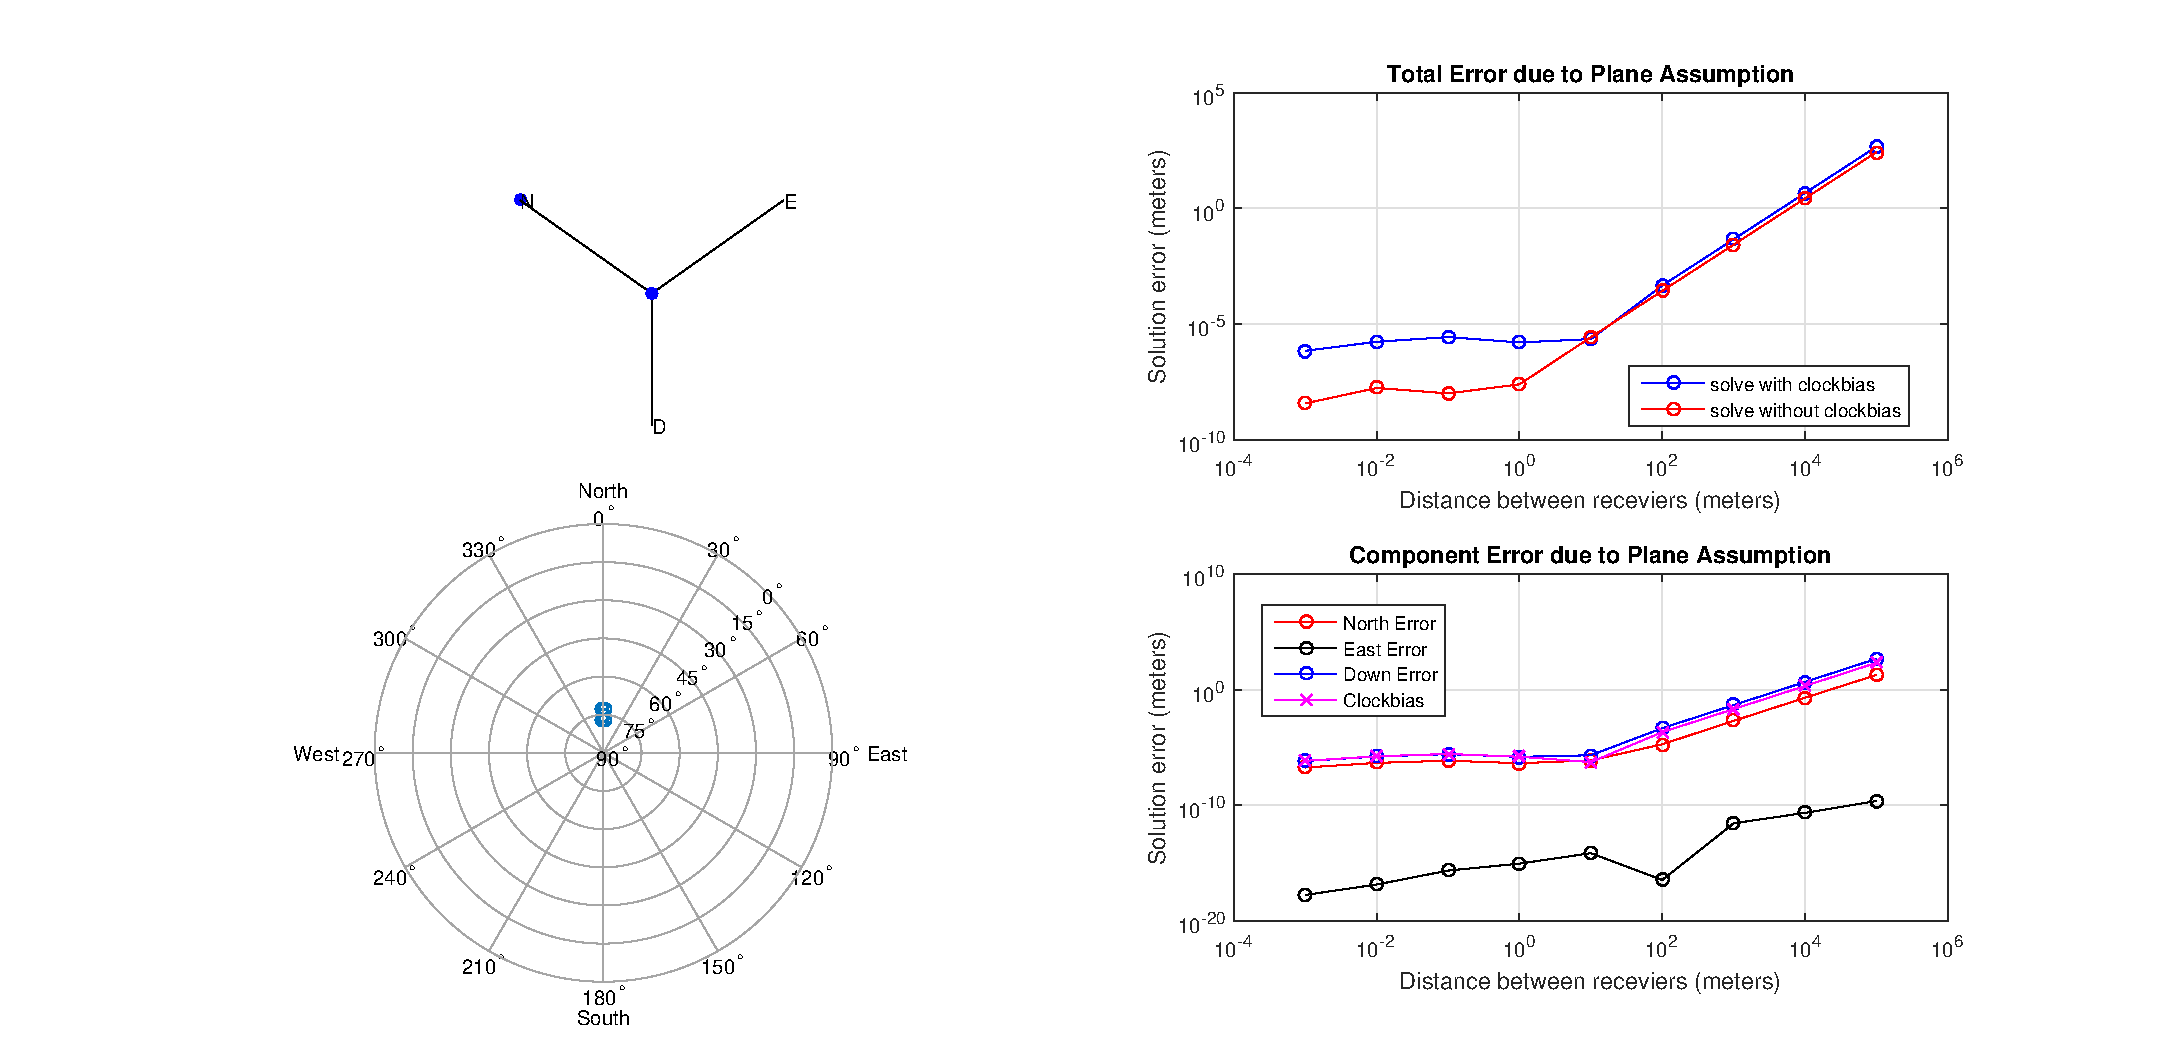
\includegraphics[trim = 3cm 0 0 0,clip,width=\linewidth]{ChapterExperiments/Figures/plane_ALLE_north_0075}
\end{figure}

%% using main_fn_planesats
\begin{figure}
\centering
\caption{NORTH: Total Error based on satellite configuration for two receivers 10 km apart along North vector}
\label{fig:plane_total_north1_pow4}
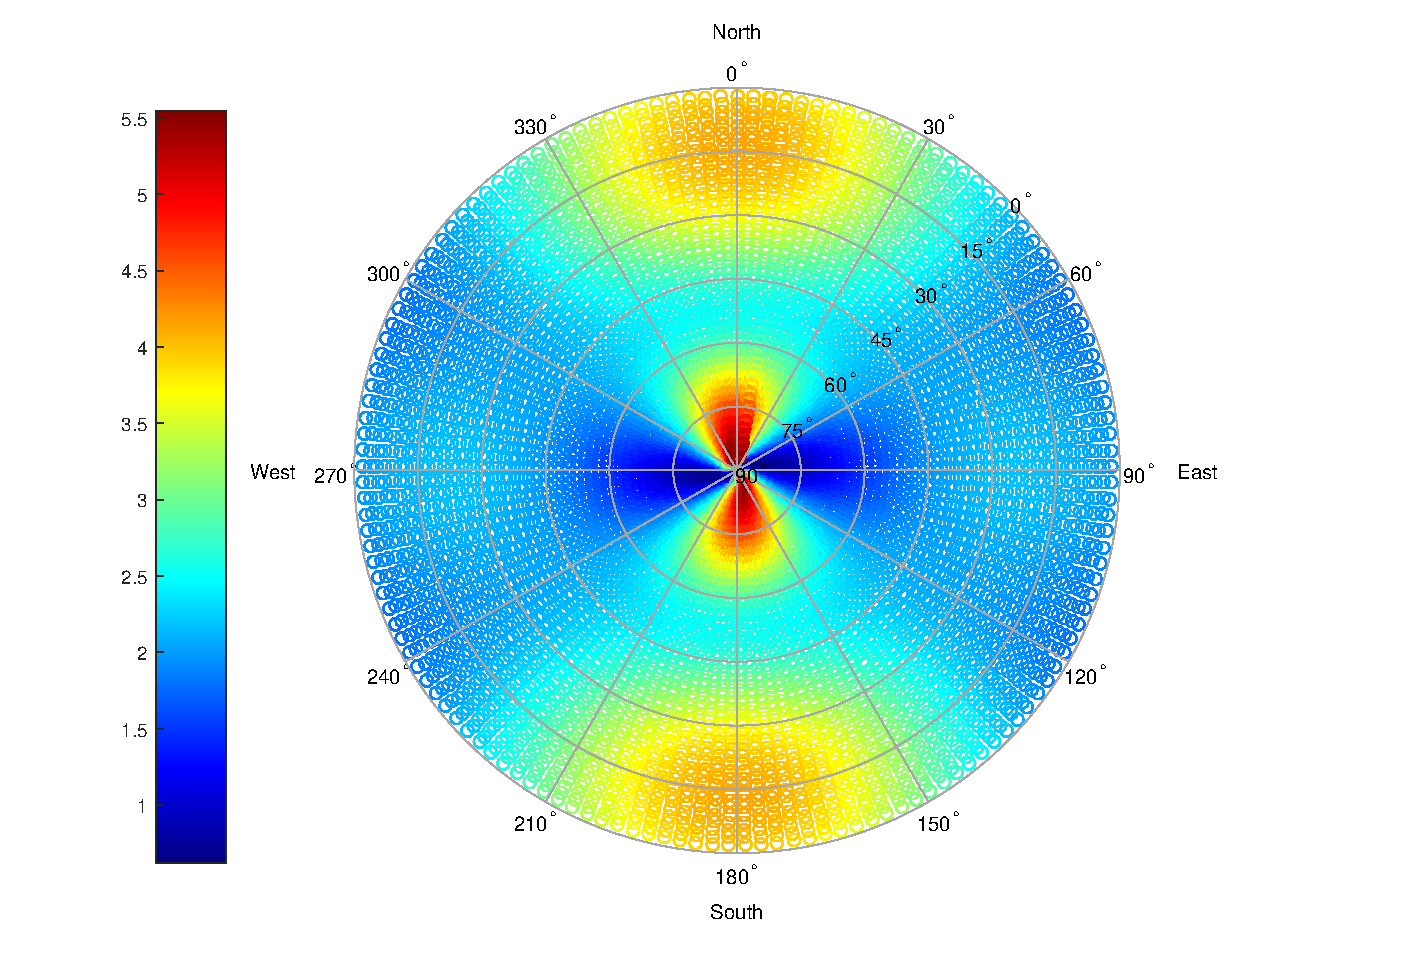
\includegraphics[width=0.7\linewidth]{ChapterExperiments/Figures/plane_total_north1_pow4}
\end{figure}

\begin{figure}
\centering
\caption{EAST: Total Error based on satellite configuration for two receivers 10 km apart along East vector}
\label{fig:plane_total_east_pow4}
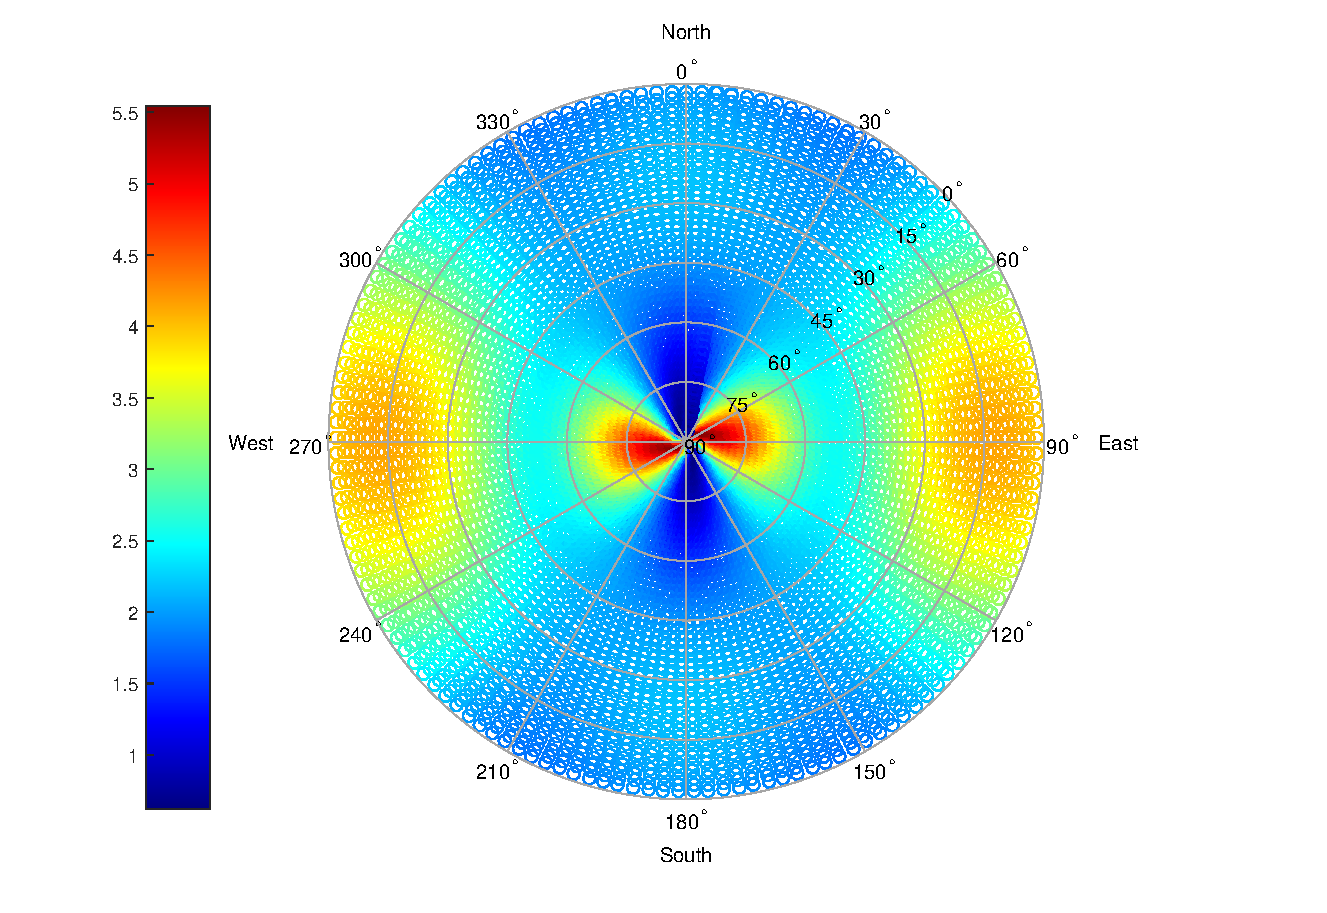
\includegraphics[width=0.7\linewidth]{ChapterExperiments/Figures/plane_total_east_pow4}
\end{figure}

\begin{figure}
\centering
\caption{DOWN: Total Error based on satellite configuration for two receivers 10 km apart along Down vector}
\label{fig:plane_total_down_pow4}
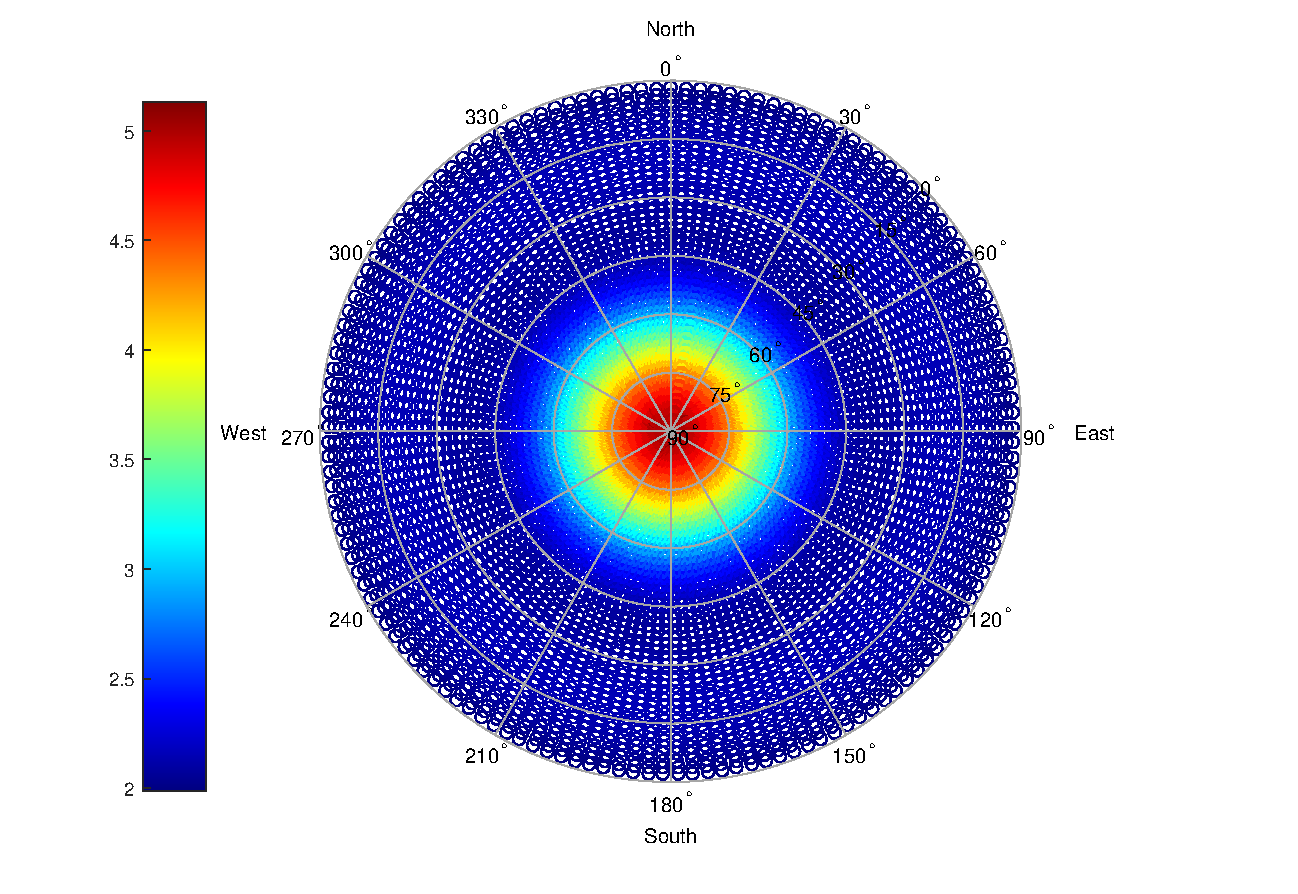
\includegraphics[width=0.7\linewidth]{ChapterExperiments/Figures/plane_total_down_pow4}
\end{figure}

\begin{figure}
\centering
\caption{Full breakdown of component error based on satellite configuration due to plane assumption (Note that not all the scales are the same but all are in meters)}
\label{fig:plane_fullbreakdown}
\begin{subfigure}[t]{0.49\textwidth}
\centering
\caption{Config:North, Error:North}
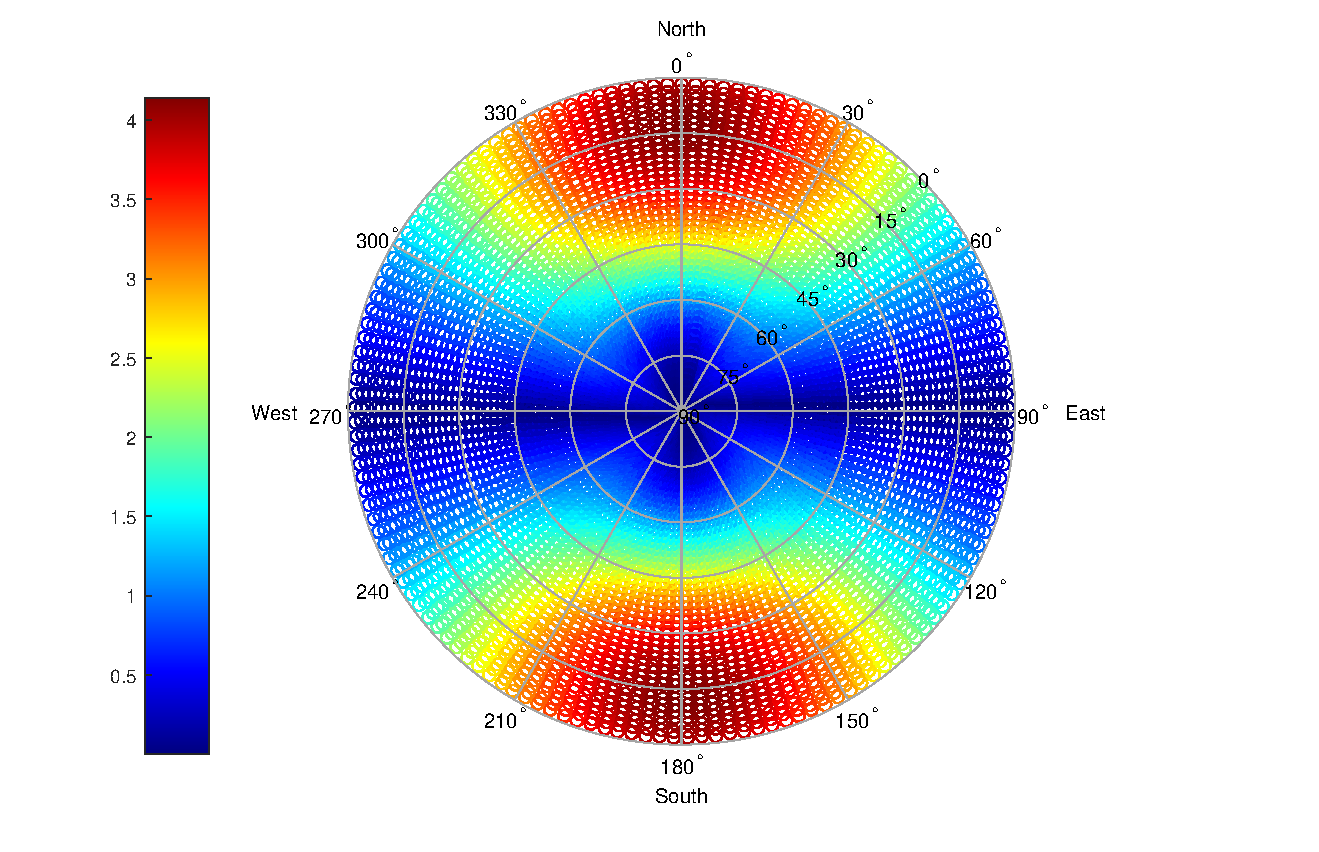
\includegraphics[width =\linewidth]{ChapterExperiments/Figures/plane_Enorth_north_pow4}
\end{subfigure}
\begin{subfigure}[t]{0.49\linewidth}
\centering
\caption{Config:Down, Error:North}
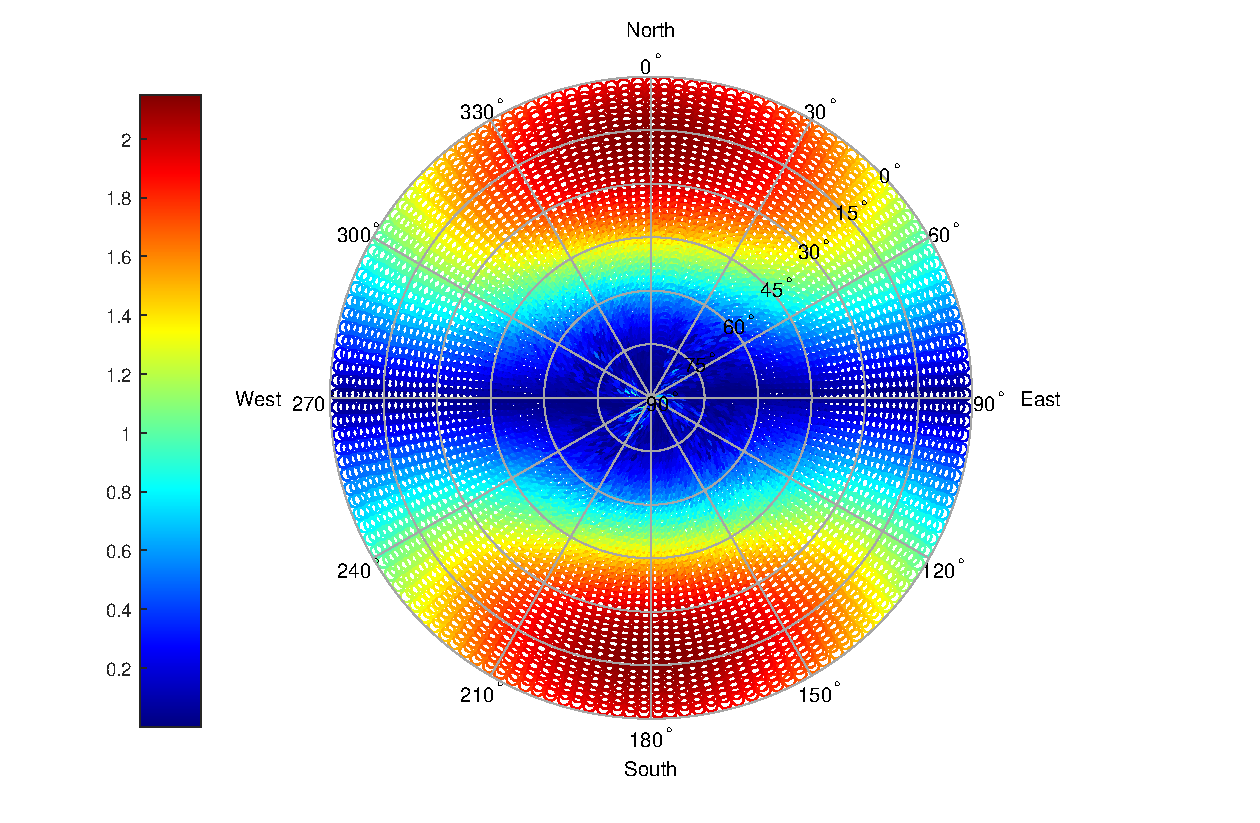
\includegraphics[width = \linewidth]{ChapterExperiments/Figures/plane_Enorth_down_pow4}
\end{subfigure}
\begin{subfigure}[t]{0.49\textwidth}
\centering
\caption{Config:North, Error:East}
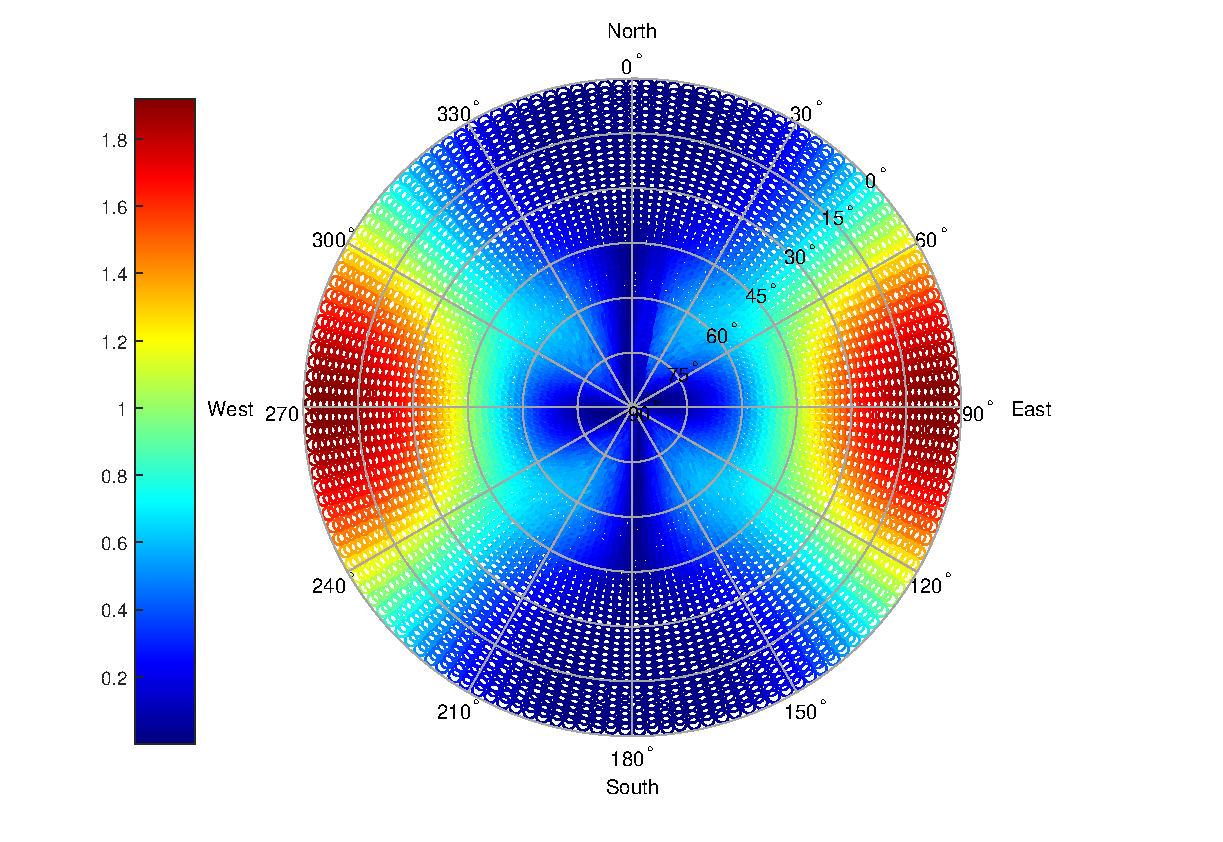
\includegraphics[width =\linewidth]{ChapterExperiments/Figures/plane_Eeast_north_pow4}
\end{subfigure}
\begin{subfigure}[t]{0.49\linewidth}
\centering
\caption{Config:Down, Error:East}
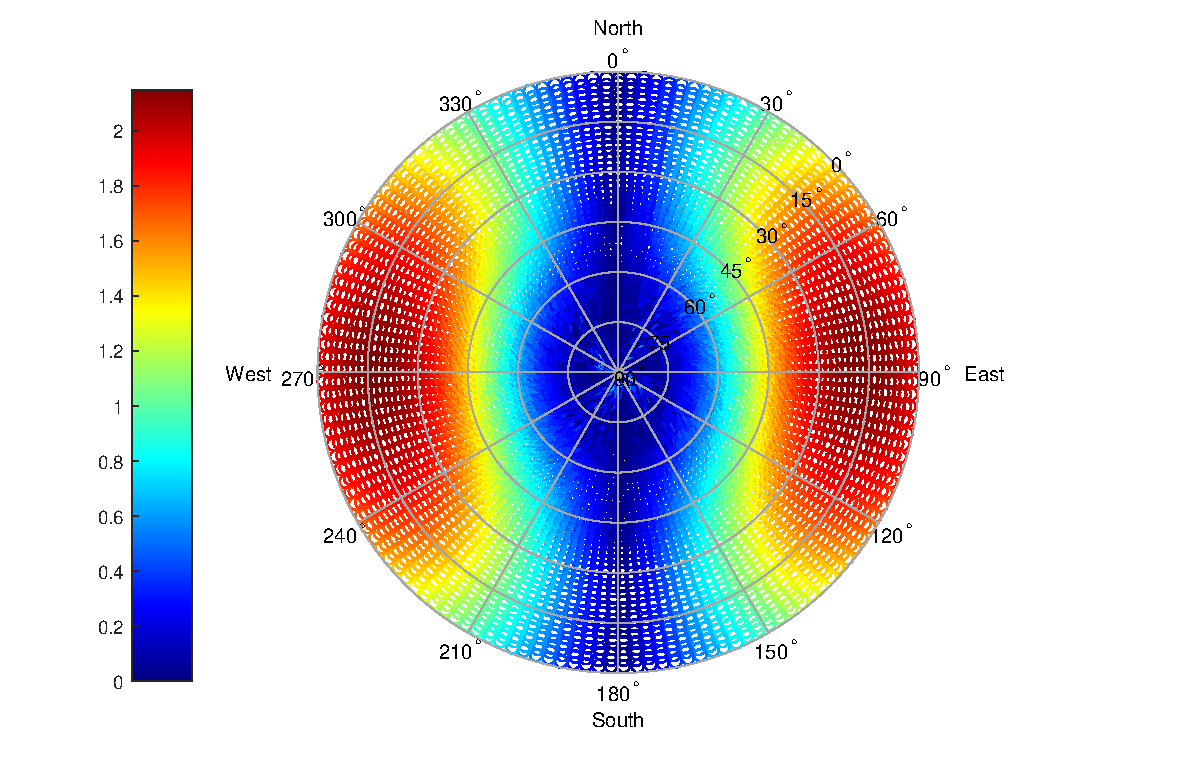
\includegraphics[width = \linewidth]{ChapterExperiments/Figures/plane_Eeast_down_pow4}
\end{subfigure}
\begin{subfigure}[t]{0.49\textwidth}
\centering
\caption{Config:North, Error:Down}
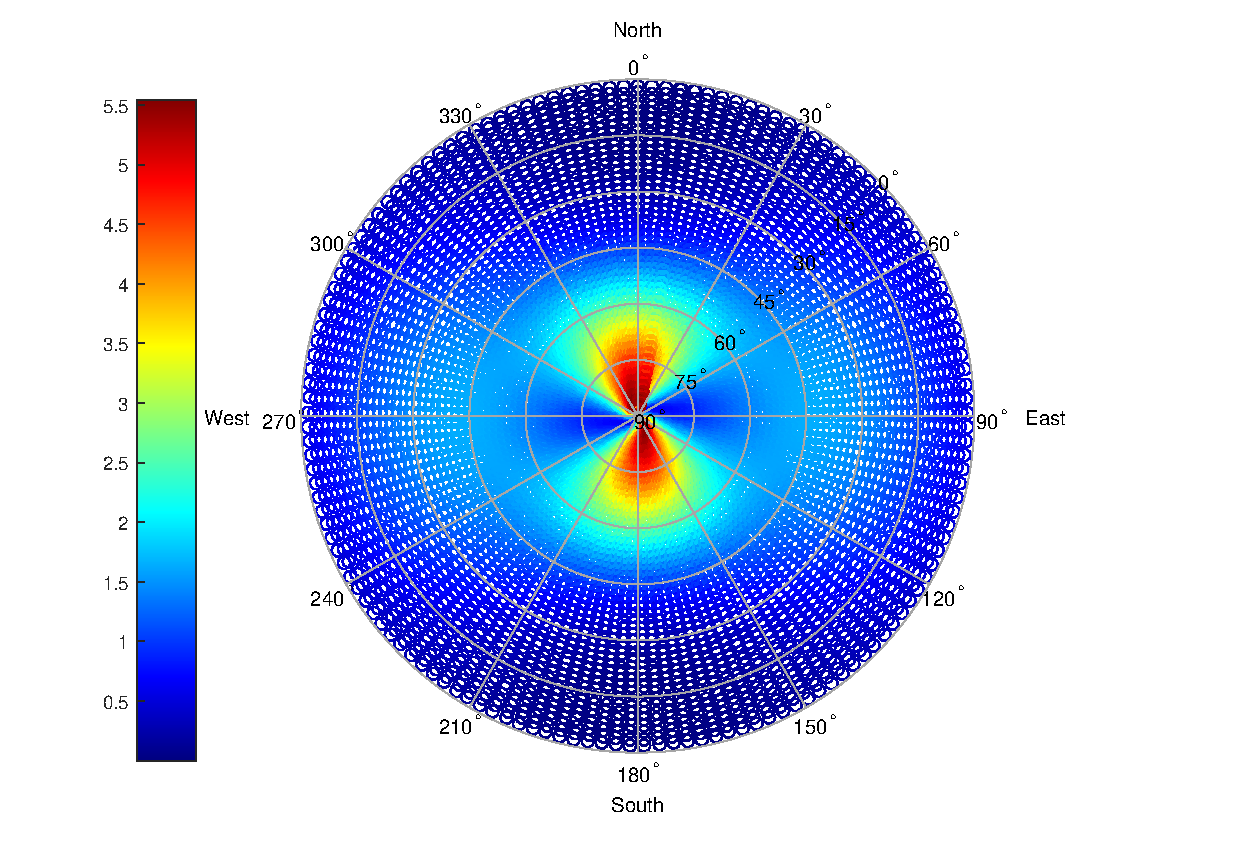
\includegraphics[width =\linewidth]{ChapterExperiments/Figures/plane_Edown_north_pow4}
\end{subfigure}
\begin{subfigure}[t]{0.49\linewidth}
\centering
\caption{Config:Down, Error:Down}
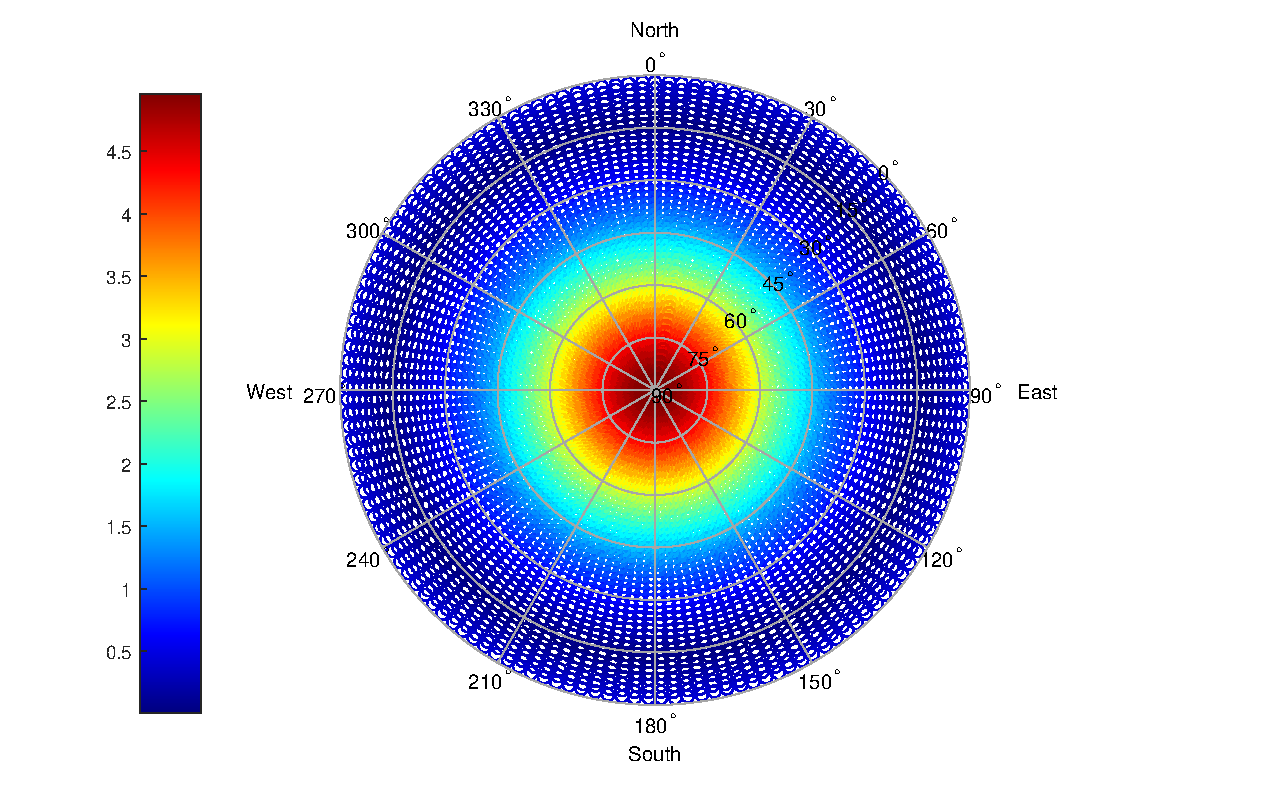
\includegraphics[width = \linewidth]{ChapterExperiments/Figures/plane_Edown_down_pow4}
\end{subfigure}
\end{figure}
